\documentclass[12pt]{article}
\usepackage[left=1in,top=1in,right=1in,bottom=1in]{geometry} 
\geometry{letterpaper} % or letter or a5paper or ... etc
\usepackage{graphicx}
%\usepackage{color}
\usepackage{longtable}


\title{CAMEO Ethnic Coding System
\thanks{ This framework was developed  with funding provided by the National Science Foundation award SES-1259190, ``Collaborative Research: Automated Real-Time Production of Political Indicators.''}}
\author{Benjamin Bagozzi and Jay Yonamine \\Pennsylvania State University}
\date{Updated for the Open Event Data Alliance\\ PLOVER Project: \today} 


\begin{document}

\pagenumbering{gobble} 
\maketitle

\begin{figure}[h!]
\centering
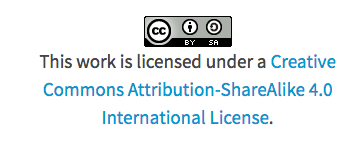
\includegraphics[width=0.6\textwidth]{cc_license}
\end{figure}

\newpage


\section{Introduction}
\label{sect:CAMEOECS}

CAMEOECS systematically assigns three-letter (lower-case) alphabetic codes to individual ethnic groups and generalized ethnic terms. It was created in 2011 as a part of a larger, CAMEO-based project, and is thus intended to serve as an optional supplement to CAMEO codes. The CAMEOECS directory includes a relatively comprehensive list of 603 ethnic groups; and a slightly less comprehensive list of each ethnic group's primary countries of settlement.  CAMEOECS is distinct from CAMEORCS in that (i) religious groups are not treated as ethnic groups by CAMEOECS (unless there is a clear ethnic dimension) and (ii) the group entries within CAMEOECS are non-hierarchical.

The three primary components of CAMEOECS are \textit{Ethnic Group Names}, \textit{Ethnic Group Codes}, and \textit{Selected Countries}.  \textit{Ethnic Group Names} reports the most common English-language name of each ethnic-group entry in CAMEOECS.  \textit{Ethnic Group Codes} provides a unique three-letter (lower case) alphabetic code for each ethnic group entry included within CAMEOECS.  \textit{Selected Countries} lists the primary countries of settlement (by UN Country Code) for each ethnic group included in CAMEOECS.  What follows is a more detailed description of each of these three components, as well as a discussion of the coding decisions that were used to create each.

\section{Identification of Ethnic Groups}\label{sect:CAMEOECSIdent}
To create a comprehensive list of ethnic groups, CAMEOECS drew from two primary sources: (1) the International Organization for Standardization's (ISO) Codes for the Representation of Names of Languages (ISO-639.2; http://www.loc.gov/standards/iso639-2/) and (2) the Ethnic Power Relations (EPR) dataset 3.1 (http://www.epr.ucla.edu/).  The creation of a CAMEOECS ethnic groups list from these two sources unfolded in the following four steps:
\begin{enumerate}
\item First, the subset of all ISO 639.2 Languages that corresponded to specific ethnic groups were identified, and this list was then used as the baseline-set of ethnic groups for inclusion in CAMEOECS.
\item ISO 639.2 Languages that did not correspond to a specific ethnic group were discarded.  Examples of ISO 639.2 Languages that were discarded include language-entries that were determined to be extinct (e.g. ``Phoenician''), artificial (e.g. ``Klingon'') or representative of general language families that encompassed multiple ethnic groups (e.g. ``Baltic languages'').
\item The ethnic groups included in the EPR 3.1 dataset were then matched by hand to the verified, ISO-639.2-derived baseline-set of ethnic group (described in step one).
\item After this matching exercise was completed, roughly 200 additional ethnic groups were found to uniquely exist within the EPR 3.1 dataset, and these groups were then added to the matched CAMEOECS ethnic group list to create the final CAMEOECS list of ethnic groups.
\end{enumerate}
Altogether, this coding scheme identified 603 unique ethnic groups.

\section{CAMEOECS Components}

\subsection{Ethnic Group Names}
	Each CAMEOECS ethnic group identified through the process described above was then assigned a unique \textit{Ethnic Group Name} for identification and referencing purposes.  These \textit{Ethnic Group Names}, which appear in Table \ref{tab:ECS1} below (column one), report the primary English name of each CAMEOECS ethnic group entry.  An ethnic group's ``primary'' name is defined as that group's most commonly used name within modern (spoken) English.  In order to systematically determine each ethnic group's most common (spoken) English name, an ethnic group's default Wikipedia (http://www.wikipedia.org/) name entry was used as its primary \textit{Ethnic Group Name}.  As a result, many of the \textit{Ethnic Group Names} that are used in Table \ref{tab:ECS1} differ from the names given to these ``groups'' by ISO 639.2 (which instead lists the ``English Name of Language'' corresponding to each groups) or by the EPR 3.1.  Where applicable, alternative (English-language) ethnic group names---based largely on the EPR 3.1's ethnic group name(s)---appear in parentheses after the primary \textit{Ethnic Group Name} in Table \ref{tab:ECS1} (column one).  Note however that these alternative spoken-English \textit{Ethnic Group Names} are by no means comprehensive.  Lastly, in instances where more than one ethnic group was found to use the same primary \textit{Ethnic Group Name}, groups are distinguished by the inclusion of their region of settlement within their \textit{Ethnic Group Name}.


\subsection{Ethnic Group Codes}
In addition to an \textit{Ethnic Group Name}, each ethnic group entry in Table \ref{tab:ECS1} was assigned a unique three-letter (lower case) alphabetic actor-code (column 2), hereafter referred to as \textit{Ethnic Group Code}.  Ethnic groups were assigned unique \textit{Ethnic Group Codes} based either on (i) an ethnic group's three letter (lower case) ISO 639.2 Language code (in cases where ethnic groups were found to have a matching ISO 639.2 Language in Step 1 of section \ref{sect:CAMEOECSIdent} above) or---in instances where ethnic groups did not have a matching ISO 639.2 Language code---(ii) a mnemonically assigned three letter-code derived from that group's \textit{Ethnic Group Name}.  Regarding case (i), several ISO 639.2 Languages have two unique ISO 639.2 Language code entries---one for bibliographic purposes and one for terminology purposes---and in these instances the bibliographic ISO 639.2 codes were used for \textit{Ethnic Group Name}.  Regarding case (ii), care was taken to ensure that the mnemonically assigned \textit{Ethnic Group Codes} did not conflict with any existing ISO 639.2 Language codes; including the ISO 639.2 codes for ISO 639.2 Language entries that were discarded in in Step 2 of section \ref{sect:CAMEOECSIdent} above (i.e. extinct, overly general, or artificial ISO 639.2 Languages).  Note that as a result of this latter consideration, some ethnic groups were assigned mnemonic \textit{Ethnic Group Codes} that were not the ``ideal'' mnemonic abbreviations of their corresponding \textit{Ethnic Group Name}.  In sum, the \textit{Ethnic Group Codes} in Table \ref{tab:ECS1} perfectly correspond to ISO 639.2 Language codes in instances where CAMEOECS ethnic groups have matching ISO 639.2 Languages, and distinctly correspond to newly created, mnemonic codes in instances where CAMEECS ethnic groups did not have existing ISO 639.2 Language entries.


\subsection{Selected Countries}
\textit{Selected Countries} reports the primary countries of settlement for each ethnic group entry in Table \ref{tab:ECS1}.  A ``country of settlement'' is defined as any country where an ethnic group is deemed to be politically relevant (based on the EPR 3.1's definition of political relevancy) or have a sizable population (roughly greater than 1,000 ethnic group members).\footnote{According to the EPR 3.1. codebook (pg. 2), ``An ethnic category is politically relevant if at least one significant political actor claims to represent the interests of that group in the national political arena, or if members of an ethnic category are systematically and intentionally discriminated against in the domain of public politics. By `significant' political actor we mean a political organization (not necessarily a party) that is active in the national political arena. We define discrimination as political exclusion directly targeted at an ethnic communityóthus disregarding indirect discrimination based, for example, on educational disadvantage or discrimination in the labor or credit markets.''}  \textit{Selected Countries} are listed in Table \ref{tab:ECS1} by (comma-separated, alphabetized) United Nations Country Codes (as defined in Table \ref{tab:UNcodes}), and were collected from two primary sources.

First, all of an ethnic group's countries of relevance (for years 1946-2005) were identified within the EPR 3.1.  If a country was indicated as being a relevant for a given ethnic group---\textit{for any year within the EPR 3.1's 1946-2005 sample frame}---it was added as a \textit{Selected Country} for that ethnic group's entry in Table \ref{tab:ECS1} below.  While the EPR 3.1 deems some countries to be relevant to specific ethnic groups in some years but not others, the goal of CAMEOECS is to capture every country where an ethnic group could potentially be active, and therefore the EPR 3.1's year/relevance constraints were not applied to a given ethnic group's \textit{Selected Country} listings below.  Note that not all ethnic groups included within CAMEOECS had a matching EPR 3.1 entry, and accordingly, the use of EPR 3.1 countries of relevance in coding \textit{Selected Countries} applies to some CAMEOECS ethnic groups but not others.

Second, ethnic groups' Wikipedia entries were used to assess these groups' ``regions of significant populations.''  Where these regions were listed with specific population numbers, any country with greater than 1,000 members of a given ethnic group was included as a \textit{Selected Country} for that ethnic group in Table \ref{tab:ECS1}.  Note that this coding scheme has a moderate bias towards large developed countries with significant histories of immigration (e.g. Australia, France, the United States of America).  For Wikipedia entries that did not report specific population numbers, or that did not contain a ``regions of significant populations'' section at all, any country included on that ethnic group's Wikipedia page was added as a \textit{Selected Country} for that group.  Note that, irrespective of whether a given ethnic group had a ``regions of significant populations'' section or not, Wikipedia entries for ethnic groups were often incomplete and are thus likely missing many countries with significant populations of CAMEOECS ethnic groups. \textit{Selected Country} is therefore very much a work-in-progress.  Also note that the use of ethnic groups' Wikipedia page entries to code \textit{Selected Countries} was applied \textit{both} to groups that had no relevant-country entries in the EPR 3.1 \textit{and} to ethnic groups with relevant countries listed by the EPR 3.1. Regarding the latter, there was often a high degree of correspondence between the countries listed under Wikipedia and those included in the EPR 3.1.  However, when additional countries were listed in one source but not the other, these additional countries were always included within \textit{Selected Countries}, so as to create the most compressive list of ethnic groups' countries of settlement as was possible at this time.



\begin{center}
\begin{longtable}{|p{7cm}|p{1cm}|p{7cm}|}
\caption{CAMEO Ethnic Group Codes}
\label{tab:ECS1}
\\ \cline{1-3}
\textbf{Ethnic Group Name}  & \textbf{Code} & \textbf{Selected Countries} \\ \cline{1-3}
\hline
\endfirsthead
\hline
\textbf{Ethnic Group Name}  & \textbf{Code} & \textbf{Selected Countries} \\ \cline{1-3}
\hline
\endhead
\hline
\multicolumn{3}{r}{\emph{continued on next page}}
\endfoot
\hline
\endlastfoot
Abkhaz (Abkhazians)	&	abk 	&	GEO, DEU, RUS, SYR, TUR, UKR	\\	\cline{1-3}
Aboriginal-Australians (Aborigines)	&	abr	&	AUS	\\	\cline{1-3}
Acehnese (Achinese)	&	ace 	&	IDN, MYS	\\	\cline{1-3}
Achang	&	acg	&	CHN, MMR	\\	\cline{1-3}
Acholi	&	ach 	&	SDN, UGA	\\	\cline{1-3}
Adivasi	&	adi	&	IND, NPL	\\	\cline{1-3}
Adjarians (Adzhars)	&	adj	&	GEO, TUR	\\	\cline{1-3}
Adyghe (Circasians)	&	ady 	&	BGR, DEU, IRQ, ISR, JOR, LBY, NLD, RUS, SYR, TUR, USA	\\	\cline{1-3}
Afar	&	aar 	&	DJI, ERI, ETH	\\	\cline{1-3}
Afrikaners	&	afr 	&	BWA, LSO, MWI, SWZ, ZAF, ZMB,  ZWE	\\	\cline{1-3}
Ahmadis	&	ahm	&	BGD, IND, IDN, PAK 	\\	\cline{1-3}
Ainu	&	ain 	&	JPN, RUS	\\	\cline{1-3}
Aja	&	aja	&	BEN, TGO	\\	\cline{1-3}
Akan (Asante)	&	aka 	&	BEN, BFA, CAN, CIV, FRA, GBR, GHA, JAM, LBR, MLI, NGA, SUR, TGO, USA	\\	\cline{1-3}
Aku (Creoles)	&	aku	&	GMB	\\	\cline{1-3}
Albanians	&	alb	&	ALB, CAN, CHE, DEU, DNK, GBR, GRC, HRV, ITA, MKD, MTN, NLD, NOR, ROM, SRB, SWE, TUR, UKR, USA	 \\	\cline{1-3}
Aleut	&	ale 	&	RUS, USA	\\	\cline{1-3}
Algonquian	&	alg 	&	USA	\\	\cline{1-3}
Altay (Altai)	&	alt 	&	RUS	\\	\cline{1-3}
Alur	&	alu	&	COD, UGA	\\	\cline{1-3}
Ambonese (Amboinese)	&	amb	&	IDN	\\	\cline{1-3}
Americo-Liberians	&	ame	&	LBR	\\	\cline{1-3}
Amhara	&	amh 	&	CAN, DJI, EGY, ERI, ETH, ISR, NOR, SDN, SOM, SWE, USA, YEM	\\	\cline{1-3}
Angika speakers	&	anp 	&	IND, NPL	\\	\cline{1-3}
Ankole	&	nyn 	&	UGA	\\	\cline{1-3}
Apache	&	apa 	&	USA	\\	\cline{1-3}
Arab	&	ara 	&	DZA, EGY, ISR, IRN, IRQ, JOR, KWT, LBN, LBY, MAR, MLI, SAU, SDN, SOM, SYR, TCD, TUN, USA, YEM	 \\	\cline{1-3}
Aragonese	&	arg 	&	ESP	\\	\cline{1-3}
Arapaho	&	arp 	&	USA	\\	\cline{1-3}
Arawak	&	arw 	&	COL, GUY, SUR, VEN 	\\	\cline{1-3}
Argentinians	&	atg	&	ARG, AUS, BOL, BRA, CAN, CHE, CHL, DEU, ESP, FRA, GBR, ISR, ITA, JPN, MEX, PER, PRY, URY, USA, VEN	\\	\cline{1-3}
Armenian	&	arm	&	ARG, ARM, AUS, AZE, BRA, CAN, CYP, FRA, GEO, GRC, RN, LBN, POL, RUS, SYR, TUR, UKR, USA	\\	 \cline{1-3}
Aromanians	&	rup 	&	ALB, BGR, GRC, MKD, ROM, SRB	\\	\cline{1-3}
Ashanti	&	twi 	&	CIV, GHA	\\	\cline{1-3}
Asian	&	asa	&	AUS, CHN, GBR, JPN, KOR, LAO, MMR, PRK, THA, UGA, USA, VNM, ZAF	\\	\cline{1-3}
Assamese	&	asm 	&	IND	\\	\cline{1-3}
Assyrian	&	asy	&	AUS, BEL, CAN, CHE, DEU, DNK, FRA, IRN, IRQ, ITA, JOR, LBN, NLD, RUS, SWE, TUR, USA	\\	 \cline{1-3}
Asturian	&	ast 	&	ESP	\\	\cline{1-3}
Atacamenos	&	ata	&	CHL	\\	\cline{1-3}
Athabaskan	&	ath 	&	CAN, USA	\\	\cline{1-3}
Australians	&	aus 	&	AUS	\\	\cline{1-3}
Austrians	&	auu	&	AUS, AUT, ARG, CAN, CHE, CZE, DEU, GBR, GRC, HUN, ITA, NZL, SWE, USA, ZAF	\\	\cline{1-3}
Awadhi	&	awa 	&	IND	\\	\cline{1-3}
Aymara	&	aym 	&	BOL, CHL, PER	\\	\cline{1-3}
Azande (Azande-Mangbetu)	&	znd 	&	CAF, COD, SDN	\\	\cline{1-3}
Azerbaijani (Azeri)	&	aze 	&	AUT, AZE, BLR, CAN, DEU, GBR, IRN, KAZ, KGZ, LVA, NLD, RUS, TUR, UKR, USA, UZB	\\	 \cline{1-3}
Baganda	&	bad 	&	CAN, GBR, SWE, UGA, ZAF, USA	\\	\cline{1-3}
Bai	&	bii	&	CHN	\\	\cline{1-3}
Bakongo	&	bkn	&	AGO, COD, COG	\\	\cline{1-3}
Bakweri	&	bkw	&	CMR	\\	\cline{1-3}
Balanta	&	bln	&	GMB, GNB, SEN	\\	\cline{1-3}
Balinese	&	ban 	&	IDN	\\	\cline{1-3}
Balkars	&	blk	&	KAZ, RUS	\\	\cline{1-3}
Baloch (Baluchis)	&	bal 	&	AFG, ARE, IRN, OMN, PAK	\\	\cline{1-3}
Bamar (Barman)	&	bmr	&	AUS, GBR, MMR, THA, SGP, MYS, GBR, AUS, USA	\\	\cline{1-3}
Bambara	&	bam 	&	BFA, GIN, MLI, NER, SEN	\\	\cline{1-3}
Bamileke	&	bai 	&	CMR	\\	\cline{1-3}
Bantu	&	bnt 	&	AGO, CMR, COD, NAM, TZA, ZAF, ZMB	\\	\cline{1-3}
Banyarwanda	&	bny	&	COD, UGA	\\	\cline{1-3}
Bari	&	bar	&	SDN	\\	\cline{1-3}
Bariba	&	brb	&	BEN	\\	\cline{1-3}
Bashkirs	&	bak 	&	BLR, KAZ, KGZ, RUS, TJK, UKR, UZB	\\	\cline{1-3}
Basoga (Bassa/Duala)	&	bas 	&	CMR, UGA	\\	\cline{1-3}
Basque	&	baq	&	ARG, CHL, CRI, CUB, BOL, BRA, ESP, FRA, MEX, URY, USA, VEN	\\	\cline{1-3}
Baster	&	bst	&	NAM	\\	\cline{1-3}
Batak	&	btk 	&	IDN	\\	\cline{1-3}
Bateke	&	bke	&	COD, COG, GAB	\\	\cline{1-3}
Beja	&	bej 	&	EGY, ERI, SDN	\\	\cline{1-3}
Belarusians (Byelorussians)	&	bel 	&	ARG, BEL, BLR, BRA, CAN, EST, GBR, ISR, KAZ, LTU, LVA, MDA, POL, RUS, UKR, USA	\\	\cline{1-3}
Bemba	&	bem 	&	ZMB	\\	\cline{1-3}
Bengali-Hindu (Bengali)	&	ben 	&	BGD, GBR, IND, NPL, MMR, MYS, PAK, SWE, THA, USA	\\	\cline{1-3}
Beni-Shugal-Gumez	&	bni	&	ETH	\\	\cline{1-3}
Berber	&	ber 	&	CAN, DZA, EGY, LBY, MAR, MLI, NER, TUN, USA	\\	\cline{1-3}
Beti-Pahuin (Beti)	&	bte	&	CMR, COG, GAB, GNQ, STP	\\	\cline{1-3}
Beydan (White Moors)	&	bey	&	DZA, LBY, MRT, MAR, TUN	\\	\cline{1-3}
Bhojpuri	&	bho 	&	FJI, GUY, IND, MUS, NPL, SUR, TTO	\\	\cline{1-3}
Bicolano	&	bik 	&	PHL	\\	\cline{1-3}
Bihari	&	bih 	&	BGD, FJI, GBR, GUY, IND, MUS, NPL, PAK, SUR, TTO, USA	\\	\cline{1-3}
Bilen	&	byn 	&	ERI	\\	\cline{1-3}
Black-African (Africans)	&	afa 	&	BRA, COL, CRI, CUB, DZA, ECU, GBR, HTI, LBY, MEX, MLI, MRT, NIC, PER, TTO, USA, VEN, ZAF, ZWE	\\	\cline{1-3}
Blang	&	blg	&	CHN, MMR, THA	\\	\cline{1-3}
Bodo	&	bod	&	IND	\\	\cline{1-3}
Bolivia	&	bol	&	BOL, CHL, PER, PRY	\\	\cline{1-3}
Bonan	&	bon	&	CHN	\\	\cline{1-3}
Bosniaks	&	bos 	&	AUS, AUT, BEL, BIH, DEU, DNK, HRV, ITA, MKD, MTN, NOR, SRB, SVN, SWE, TUR, USA	\\	 \cline{1-3}
Brahui	&	brh	&	AFG, IRN, PAK	\\	\cline{1-3}
Breton	&	bre 	&	CAN, FRA	\\	\cline{1-3}
Brijwasi	&	bra 	&	IND	\\	\cline{1-3}
Bugis	&	bug 	&	IDN, MYS, SGP	\\	\cline{1-3}
Bulgarian	&	bul 	&	ALB, ARE, AUT, BEL, BGR, CAN, CZE, DEU, ESP, FRA, GBR, GRC, HUN, ITA, KAZ, MDA, PRT, ROM, RUS, SRB, TUR, UKR, ZAF	\\	\cline{1-3}
Burakumin	&	brk	&	JPN	\\	\cline{1-3}
Buryat	&	bua 	&	KAZ, MNG, RUS, UZB, UKR	\\	\cline{1-3}
Bushmen (San)	&	bsh	&	BWA, NAM, ZAF	\\	\cline{1-3}
Buyei	&	bou	&	CHN, VNM	\\	\cline{1-3}
Cabindan-Mayombe	&	cab	&	AGO	\\	\cline{1-3}
Caddo	&	cad 	&	USA	\\	\cline{1-3}
Cape Verdean	&	cap	&	CPV, GNB	\\	\cline{1-3}
Catalan	&	cat 	&	AND, ARG, CHL, CUB, DEU, ESP, FRA, ITA, MEX, VEN	\\	\cline{1-3}
Caucasian Avars (Avars)	&	ava 	&	AZE, GEO, RUS	\\	\cline{1-3}
Cebuano	&	ceb 	&	PHL	\\	\cline{1-3}
Chagatai	&	chg 	&	UZB	\\	\cline{1-3}
Cham 	&	cmc 	&	FRA, KHM, LAO, MYS, THA, USA, VNM	\\	\cline{1-3}
Chamorro	&	cha 	&	FSM, MNP, USA	\\	\cline{1-3}
Chechen	&	che 	&	AZE, EGY, GEO, IRN, IRQ, JOR, KAZ, RUS, SYR, TUR	\\	\cline{1-3}
Cherokee	&	chr 	&	USA	\\	\cline{1-3}
Chewa	&	chw	&	MWI	\\	\cline{1-3}
Chewa (Nyanja speakers)	&	nya 	&	MOZ, MWI, ZMB, ZWE	\\	\cline{1-3}
Cheyenne	&	chy 	&	USA	\\	\cline{1-3}
Chileans	&	chl	&	ARG, BRA, CHL, DEU, ESP, FRA, SWE, USA, VEN	\\	\cline{1-3}
Chinese (Mainland Chinese)	&	chi	&	AUS, BRA, CAN, CHN, ESP, FRA, GBR, IDN, IND, ITA, KHM, KOR, LAO, MMR, MYS, NLD, NZL, PER, PHL, PRK, SGP, THA, USA, VNM, ZAF	\\	\cline{1-3}
Chinook	&	chn 	&	USA	\\	\cline{1-3}
Chipewyan	&	chp 	&	CAN	\\	\cline{1-3}
Choctaw	&	cho 	&	USA	\\	\cline{1-3}
Ch'orti' (Chorti)	&	cht	&	GTM, HND	\\	\cline{1-3}
Chukchi	&	chc	&	RUS	\\	\cline{1-3}
Chuukese	&	chk 	&	FSM	\\	\cline{1-3}
Chuvash	&	chv 	&	BLR, KAZ, KGZ, MDA, RUS, TKM, UZB	\\	\cline{1-3}
Colombian	&	col	&	ARG, AUS, BRA, CAN, COL, CRI, ESP, GBR, ISR, ITA, MEX, USA, VEN	\\	\cline{1-3}
Cook Islands Maori	&	rar 	&	COK, NZL	\\	\cline{1-3}
Cornish	&	cor 	&	AUS, CAN, GBR, MEX, NZL, USA, ZAF	\\	\cline{1-3}
Corsican	&	cos 	&	FRA	\\	\cline{1-3}
Costa Ricans	&	csr	&	CRI, NIC, PAN	\\	\cline{1-3}
Cotiers	&	cot	&	MDG	\\	\cline{1-3}
Cree	&	cre 	&	CAN, USA	\\	\cline{1-3}
Creole	&	crp 	&	BLZ, CPV, DMA, GLP, GMB, GNB, GNQ, HTI, JAM, LCA, MTQ, NGA, SEN, SLE, STP, TTO	\\	\cline{1-3}
Crimean Tatar	&	crh 	&	BGR, ROM, TUR, UKR, UZB	\\	\cline{1-3}
Croats	&	hrv 	&	ARG, AUS, AUT, BIH, CAN, CHE, CHL, DEU, DNK, FRA, HRV, HUN, ITA, MTN, NOR, ROM, SRB, SVN, SWE, USA, ZAF	\\	\cline{1-3}
Cushitic	&	cus 	&	EGY, KEN, SDN, SOM, TZA	\\	\cline{1-3}
Czech	&	cze	&	ARG, AUS, AUT, BRA, CAN, CHE, CZE, DEU, ESP, FRA, GBR, HRV, ISR, IRL, ITA, MEX, NLD, POL, ROM, RUS, SRB, SVK, SVN, SWE, UKR, USA, ZAF	\\	\cline{1-3}
Dai	&	dai	&	CHN, LAO, THA	\\	\cline{1-3}
Dalit (Backward classes/castes)	&	dal	&	BGD, IND, LKA, NPL, PAK	\\	\cline{1-3}
Damara	&	dam	&	NAM	\\	\cline{1-3}
Danes	&	dan 	&	AUS, AUT, BRA, CAN, CHE, DEU, DNK, ESP, FRA, GBR, IRL, ISL, NOR, NZL, SWE, USA	\\	\cline{1-3}
Dargwa (Dargins)	&	dar 	&	RUS	\\	\cline{1-3}
Daur	&	dau	&	CHN	\\	\cline{1-3}
Dayak	&	day 	&	BRN, IDN, MYS	\\	\cline{1-3}
Dinka	&	din 	&	SDN	\\	\cline{1-3}
Djerma-Songhai	&	dje	&	NER	\\	\cline{1-3}
Dogras	&	doi 	&	IND, PAK	\\	\cline{1-3}
Dogrib	&	dgr 	&	CAN	\\	\cline{1-3}
Dominicans	&	dom	&	DOM, HTI, USA	\\	\cline{1-3}
Dong	&	don	&	CHN, VNM	\\	\cline{1-3}
Dongxiang	&	dox	&	CHN	\\	\cline{1-3}
Dravidian	&	dra 	&	IND, LKA, PAK	\\	\cline{1-3}
Druze	&	dru	&	AUS, CAN, ISR, JOR, LBN, SYR, USA, VEN	\\	\cline{1-3}
Duala	&	dua 	&	CMR	\\	\cline{1-3}
Dutch (Flemings)	&	dut	&	AUS, CAN, BEL, BRA, NLD, NZL, USA, ZAF	\\	\cline{1-3}
Dyula	&	dyu 	&	BFA, GNB, MLI, SEN	\\	\cline{1-3}
East Indian	&	ein	&	MYS, TTO	\\	\cline{1-3}
East Timorese	&	eat	&	IDN, TMP	\\	\cline{1-3}
Ecuadorians	&	ecu	&	CHL, COL, ECU, ESP, PER, PRY, USA, VEN	\\	\cline{1-3}
Edo	&	bin 	&	NGA	\\	\cline{1-3}
Efik	&	efi 	&	CMR, NGA	\\	\cline{1-3}
Ekajuk	&	eka 	&	NGA	\\	\cline{1-3}
English	&	eng 	&	CAN, GBR, IRL, NZL, ZAF	\\	\cline{1-3}
English-Creole	&	cpe 	&	BLZ, JAM, NGA, SLE	\\	\cline{1-3}
Eshira (Bapounou)	&	esh	&	GAB	\\	\cline{1-3}
Estonian	&	est 	&	BEL, CAN, EST, FIN, GBR, IRL, LVA, NOR, RUS, SWE, UKR, USA	\\	\cline{1-3}
Europeans	&	eur	&	ZWE	\\	\cline{1-3}
Evenks	&	eve	&	CHN, RUS	\\	\cline{1-3}
Ewe	&	ewe 	&	BEN, GHA, TGO	\\	\cline{1-3}
Ewondo	&	ewo 	&	CMR	\\	\cline{1-3}
Fang (Estuary Fang)	&	fan 	&	COG, GAB, GNQ	\\	\cline{1-3}
Fante	&	fat 	&	GHA	\\	\cline{1-3}
Faroese	&	fao 	&	DNK, ISL, NOR	\\	\cline{1-3}
Fijian	&	fij 	&	AUS, FJI, GBR, NZL, USA	\\	\cline{1-3}
Filipino	&	fil 	&	ARE, AUS, CAN, CHN, ESP, ISR, ITA, JPN, KOR, KWT, MYS, NGA, NLD, NOR, NZL, PAK, PHL, QAT, SAU, USA	\\	\cline{1-3}
Finno-Ugric	&	fiu 	&	CAN, EST, FIN, HUN, NZL, ROM, RUS, SVK, SWE, USA	\\	\cline{1-3}
Finns	&	fin 	&	ARE, AUS, CAN, CHE, DEU, DNK, ESP, EST, FIN, FRA, NLD, NOR, RUS, SWE, USA	\\	\cline{1-3}
Fon	&	fon 	&	BEN, NGA	\\	\cline{1-3}
French	&	fre	&	BEL, BRA, CAN, CHE, FRA, GBR, USA	\\	\cline{1-3}
French-Creole	&	cpf 	&	DMA, GLP, HTI, LCA, MTQ, TTO	\\	\cline{1-3}
Frisians	&	frr 	&	DEU	\\	\cline{1-3}
Friulan	&	fur 	&	ITA	\\	\cline{1-3}
Fula (Fulani)	&	ful 	&	BEN, BFA, CAF, CIV, CMR, GIN, GMB, GNB, LBR, MRT, NER, NGA, SDN, SEN, SLE, TCD, TGO	\\	 \cline{1-3}
Fur	&	fru	&	SDN	\\	\cline{1-3}
Ga (Ga-Adangbe)	&	ada 	&	CAN, DEU, GBR, GHA, TGO, USA	\\	\cline{1-3}
Gaels	&	gla 	&	GBR, IRL	\\	\cline{1-3}
Galician	&	glg 	&	AND, ARG, BRA, CHE, CUB, DEU, ESP, FRA, GBR, MEX, NLD, PRT, URY, USA, VEN	\\	\cline{1-3}
Garifuna (Garifs)	&	gar	&	BLZ, GTM, HND, NIC	\\	\cline{1-3}
Gayo	&	gay 	&	IDN	\\	\cline{1-3}
Gbaya (Baya)	&	gba 	&	CAF, CMR, COD, COG	\\	\cline{1-3}
Gelao (Gelo)	&	gel	&	CHN	\\	\cline{1-3}
Georgian	&	geo	&	ARM, AZE, BRA, CAN, FRA, GBR, GEO, GRC, ISR, ITA, KAZ, RUS, SGP, TUR, UKR, USA	\\	\cline{1-3}
German	&	ger	&	ARG, AUS, AUT, BEL, BOL, BRA, CAN, CHE, CZE, DEU, DNK, ECU, ESP, FRA, GBR, GRC, HUN, ISR, ITA, KAZ, NAM, NOR, POL, ROM, RUS, URY, ZAF	\\	\cline{1-3}
Gia Rai	&	gia	&	VNM	\\	\cline{1-3}
Gin (Jing)	&	gin	&	CHN	\\	\cline{1-3}
Gio	&	gio	&	CIV, LBR	\\	\cline{1-3}
Gondi	&	gon 	&	IND	\\	\cline{1-3}
Gorontalonese (Gorontalos)	&	gor 	&	IDN	\\	\cline{1-3}
Grassfielders 	&	gra	&	CMR	\\	\cline{1-3}
Grebo	&	grb 	&	CIV, LBR	\\	\cline{1-3}
Greek	&	gre	&	ALB, ARG, AUS, BEL, BRA, CAN, CHE, CYP, DEU, FRA, GBR, GER, GRC, KAZ, ROM, RUS, SWE, UKR, USA, UZB	 \\	\cline{1-3}
Guan	&	gun	&	GHA	\\	\cline{1-3}
Guarani	&	grn 	&	ARG, BOL, BRA, PRY	\\	\cline{1-3}
Guatemalan	&	gua	&	BLZ, CRI, GTM, HND, MEX, NIC, USA	\\	\cline{1-3}
Gujarati	&	guj 	&	AUS, CAN, GBR, IND, KEN, MDG, MUS, MWI, MYS, SGP, TTO, TZA, UGA, USA, ZAF	\\	\cline{1-3}
Gwich'in	&	gwi 	&	CAN, USA	\\	\cline{1-3}
Hadjerai	&	had	&	TCD	\\	\cline{1-3}
Haida	&	hai 	&	CAN, USA	\\	\cline{1-3}
Haitian	&	hat 	&	DOM,  ESP, FRA, HTI, USA	\\	\cline{1-3}
Hani	&	hni	&	CHN, VNM	\\	\cline{1-3}
Harari	&	har	&	ETH	\\	\cline{1-3}
Haratin (Black Moors)	&	hrt	&	MRT, MAR	\\	\cline{1-3}
Hausa (Hausa-Fulani)	&	hau 	&	BEN, BFA, CIV, CMR, ERI, GHA, NER, NGA, SDN, TCD, TGO	\\	\cline{1-3}
Hawaiian	&	haw 	&	USA	\\	\cline{1-3}
Hazara	&	haz	&	AFG, PAK	\\	\cline{1-3}
Herero	&	her 	&	AGO, BWA, NAM	\\	\cline{1-3}
Hiligayon	&	hil 	&	PHL	\\	\cline{1-3}
Hill Tribes	&	hgh	&	MDG, THA	\\	\cline{1-3}
Himachali	&	him 	&	IND	\\	\cline{1-3}
Hiri Motu	&	hmo 	&	PNG	\\	\cline{1-3}
Hmong	&	hmn 	&	AUS, CAN, CHN, DEU, FRA, LAO, THA, USA, VNM	\\	\cline{1-3}
Hoa	&	hoa	&	VNM	\\	\cline{1-3}
Hondurans	&	hon	&	GTM, HND, MEX, SLV, USA	\\	\cline{1-3}
Hui	&	hui	&	CHN	\\	\cline{1-3}
Hungarian	&	hun 	&	BRA, CAN, CHL, CZE, GBR, HRV, HUN, IRL, MKD, ROM, RUS, SRB, SVK, SVN, TUR, UKR, USA	\\	 \cline{1-3}
Hupa	&	hup 	&	USA	\\	\cline{1-3}
Hutu	&	hut	&	BDI, COD, RWA	\\	\cline{1-3}
Iban	&	iba 	&	IDN	\\	\cline{1-3}
Icelanders	&	ice	&	CAN, ISL, NOR, USA	\\	\cline{1-3}
Igbo	&	ibo 	&	CMR, GBR, GHA, GNQ, JAM, JPN, NGA, SLE, TTO, USA	\\	\cline{1-3}
Ijaw	&	ijo 	&	NGA	\\	\cline{1-3}
Ilocono	&	ilo 	&	PHL, USA	\\	\cline{1-3}
Indian	&	idn	&	ARE, AUS, BHR, CAN, FRA, GBR, GUY, IND, KWT, MMR, MUS, NPL, SGP, OMN, SAU, USA, TTO, ZAF	\\	 \cline{1-3}
Indigenous	&	idg	&	PHL, MEX, COL, ECU, LBR, CAN, USA	\\	\cline{1-3}
Indonesian	&	ind 	&	ARE, AUS, CAN, IDN, JPN, KOR, MYS, NLD, PHL, SAU, SGP, SUR, USA	\\	\cline{1-3}
Ingush	&	inh 	&	KAZ, RUS, TUR	\\	\cline{1-3}
Inuit	&	iku 	&	CAN	\\	\cline{1-3}
Inupiat	&	ipk 	&	CAN, USA	\\	\cline{1-3}
Iranian	&	ira 	&	ARE, AUS,AUT, CAN, CHE, BHR, DEU, DNK, ESP, FRA, GBR, IRN, ISR, ITA, JPN, KWT, MYS, NLD, NOR, PHL, RUS, TUR, SWE, USA	\\	\cline{1-3}
Irish	&	gle 	&	ARG, AUS, CAN, GBR, IRL, MEX	\\	\cline{1-3}
Iroquois	&	iro 	&	CAN, USA	\\	\cline{1-3}
Itallian	&	ita 	&	AUT, CHE, DEU, ESP, FRA, HRV, ITA, SVN, USA	\\	\cline{1-3}
Japanese	&	jpn 	&	ARG, AUS, BOL, BRA, CAN, CHL, CHN, DEU, FSM, GBR, IDN, ITA, JPN, KOR, MEX, NZL, PER, PHL, PRY, SGP, THA, USA, VNM	\\	\cline{1-3}
Javanese	&	jav 	&	IDN, MYS, NLD, SUR	\\	\cline{1-3}
Jewish	&	jew	&	ARG, CAN, ISR, IRN, POL, RUS, USA	\\	\cline{1-3}
Jino (Jinuo)	&	jin	&	CHN	\\	\cline{1-3}
Jola (Diola)	&	jol	&	GMB, GNB, SEN	\\	\cline{1-3}
Kabarday (Kabardins)	&	kbd 	&	GEO, JOR, RUS, TUR	\\	\cline{1-3}
Kabye (Kabre)	&	kby	&	TGO	\\	\cline{1-3}
Kabyle	&	kab 	&	CAN, DZA, FRA, USA	\\	\cline{1-3}
Kachin	&	kac 	&	CHN, IND, MMR	\\	\cline{1-3}
Kadazan	&	kad	&	MYS	\\	\cline{1-3}
Kakwa-Nubian	&	kak	&	UGA	\\	\cline{1-3}
Kalaallit	&	kal 	&	DNK	\\	\cline{1-3}
Kali'na	&	car 	&	BRA, GUY, SUR, VEN	\\	\cline{1-3}
Kalmyk	&	xal 	&	CHN, MNG, RUS	\\	\cline{1-3}
Kamba	&	kam 	&	KEN	\\	\cline{1-3}
Kannada	&	kan 	&	IND	\\	\cline{1-3}
Kanuri (Kanouri)	&	kau 	&	CMR, NER, NGA, TCD	\\	\cline{1-3}
Kaonde	&	kao	&	COD, ZMB	\\	\cline{1-3}
Kapampangan	&	pam 	&	CAN, PHL, USA	\\	\cline{1-3}
Karachays (Karachai)	&	kch	&	KAZ, RUS, SYR, TUR, USA	\\	\cline{1-3}
Karakalpak	&	kaa 	&	KAZ, RUS, TKM, TUR, UZB	\\	\cline{1-3}
Karamojong	&	krm	&	UGA	\\	\cline{1-3}
Karelians	&	krl 	&	BLR, EST, FIN, RUS	\\	\cline{1-3}
Karen (Kayin)	&	kar 	&	MMR, THA	\\	\cline{1-3}
Kashmiri	&	kas 	&	GBR, IND, PAK	\\	\cline{1-3}
Kashubian	&	csb 	&	CAN, DEU, POL	\\	\cline{1-3}
Kavango	&	kav	&	NAM	\\	\cline{1-3}
Kazakhs	&	kaz 	&	CHN, DEU, IRN, KAZ, KGZ, MNG, RUS, TKM, UKR, UZB	\\	\cline{1-3}
Khakas	&	khk	&	RUS	\\	\cline{1-3}
Khasi	&	kha 	&	IND	\\	\cline{1-3}
Khmer (Khmer Loei)	&	khm 	&	AUS, BEL, CAN, FRA, KHM, KOR, LAO, MYS, NZL, THA, USA, VNM	\\	\cline{1-3}
Khmu	&	khu	&	CHN, LAO, MMR, THA, USA, VNM	\\	\cline{1-3}
Khoikhoi	&	khi 	&	NAM, ZAF	\\	\cline{1-3}
Kikuyu 	&	kik 	&	KEN	\\	\cline{1-3}
Kinyarwanda Speakers	&	kin	&	COD	\\	\cline{1-3}
Kiribati	&	gil 	&	FJI, KIR, MHL, NRU, SLB, TUV, VUT	\\	\cline{1-3}
Kisii	&	kis	&	KEN	\\	\cline{1-3}
Kokani	&	kok 	&	IND	\\	\cline{1-3}
Komi (Komi-Permyaks)	&	kom 	&	RUS	\\	\cline{1-3}
Kongo (Bakongo)	&	kon 	&	AGO, COD, COG	\\	\cline{1-3}
Kono	&	kno	&	SLE	\\	\cline{1-3}
Korean	&	kor 	&	ARG, AUS, BRA, CAN, CHN, DEU, FRA, GBR, IDN, IND, JPN, KAZ, KGZ, KHM, KOR, MYS, NZL, PHL, PRK, RUS, SGP, THA, UKR, USA, UZB, VNM	\\	\cline{1-3}
Kosraean	&	kos 	&	FSM	\\	\cline{1-3}
Kouyou	&	kou	&	COG	\\	\cline{1-3}
Kpelle (Guerze)	&	kpe 	&	GHA, LBR	\\	\cline{1-3}
Krahn (Guere)	&	krh	&	LBR	\\	\cline{1-3}
Kru	&	kro 	&	CIV, LBR	\\	\cline{1-3}
Ktunaxa	&	kut 	&	CAN, USA	\\	\cline{1-3}
Kumyks	&	kum 	&	RUS	\\	\cline{1-3}
Kurd	&	kur 	&	ARM, AZE, DEU, FRA, GBR, IRN, IRQ,  ISR, LBN, NLD, SWE, SYR, TKM, TUR	\\	\cline{1-3}
Kurichiya (Hill Barhmins)	&	brm	&	IND, NPL	\\	\cline{1-3}
Kurukh	&	kru 	&	BGD, IND	\\	\cline{1-3}
Kwanyama	&	kua 	&	AGO, NAM	\\	\cline{1-3}
Kyrgyz (Kirghis/Kirgiz)	&	kir 	&	CHN, KGZ, RUS, TJK, TUR, UKR, UZB	\\	\cline{1-3}
Lahu	&	lhu	&	CHN, LAO, MMR, THA, VNM	\\	\cline{1-3}
Lak (Russia)	&	lak	&	RUS	\\	\cline{1-3}
Lamba	&	lam 	&	BEN, TGO	\\	\cline{1-3}
Lao	&	lao 	&	CHN, KHM, LAO, MMR, MYS, THA, VNM	\\	\cline{1-3}
Lari	&	lar	&	COG	\\	\cline{1-3}
Latinos	&	ltn	&	CAN, USA	\\	\cline{1-3}
Latoka	&	ltk	&	SDN	\\	\cline{1-3}
Latvian	&	lav 	&	BRA, CAN, DEU, ESP, EST, GBR, IRL, KAZ, LTU, LVA, NOR, NZL, RUS, SWE, UKR, USA	\\	\cline{1-3}
Lenape	&	del 	&	CAN, USA	\\	\cline{1-3}
Lenca	&	len	&	HND, SLV	\\	\cline{1-3}
Lezgian (Lezgins)	&	lez 	&	AZE, RUS	\\	\cline{1-3}
Li	&	lii	&	CHN	\\	\cline{1-3}
Limba	&	lba	&	CMR, SLE	\\	\cline{1-3}
Limburgian	&	lim 	&	BEL, DEU, NLD	\\	\cline{1-3}
Lingala	&	lin 	&	COD, COG	\\	\cline{1-3}
Lisu	&	lsu	&	CHN, IND, MMR, THA	\\	\cline{1-3}
Lithuanian	&	lit 	&	AUT, BLR, BRA, CAN, DEU, ESP, FRA, IRL, ISL, LTU, LVA, POL, RUS, USA, ZAF	\\	\cline{1-3}
Lomwe (Nguru)	&	lom	&	MOZ, MWI	\\	\cline{1-3}
Lovale	&	lov	&	AGO, ZAM	\\	\cline{1-3}
Lower Sorbian	&	dsb 	&	DEU	\\	\cline{1-3}
Lozi (Barotse)	&	loz 	&	AGO, BWA, NAM, ZMB	\\	\cline{1-3}
Luba-Kasai	&	lua 	&	COD	\\	\cline{1-3}
Luba-Katanga	&	lub 	&	COD	\\	\cline{1-3}
Lugbara	&	lgb	&	COD, UGA	\\	\cline{1-3}
Luhya	&	luh	&	KEN, TZA, UGA	\\	\cline{1-3}
Luiseno	&	lui 	&	USA	\\	\cline{1-3}
Lulua	&	lul	&	COD	\\	\cline{1-3}
Lumad	&	mno 	&	PHL	\\	\cline{1-3}
Lunda	&	lun 	&	AGO, COD, ZMB	\\	\cline{1-3}
Luo	&	luo 	&	COD, ETH, KEN, SDN, TZA, UGA 	\\	\cline{1-3}
Lusei	&	lus 	&	BGD, IND, MMR	\\	\cline{1-3}
Luxembourgers	&	ltz 	&	ARG, BEL, BRA, FRA, LUX, USA	\\	\cline{1-3}
Maasai	&	mas 	&	KEN, TZA	\\	\cline{1-3}
Macedonian	&	mac 	&	ALB, AUS, BEL, BIH, CHE, CZE, DEU, DNK, FRA, GBR, GRC, HRV, HUN, ITA, MKD, NOR, SRB, SVK, SVN, SWE, TUR, USA	\\	\cline{1-3}
Madhesi	&	mdh	&	NPL	\\	\cline{1-3}
Madi	&	mdi	&	SDN, UGA	\\	\cline{1-3}
Madurese (Madura)	&	mad 	&	IDN	\\	\cline{1-3}
Mafwe	&	maf	&	IDN, NAM	\\	\cline{1-3}
Magahi	&	mag 	&	IND	\\	\cline{1-3}
Maithili	&	mai 	&	IND, NPL	\\	\cline{1-3}
Makassarese	&	mak 	&	IDN	\\	\cline{1-3}
Makonde (Makonde-Yao)	&	mok	&	MOZ, TZA	\\	\cline{1-3}
Malagasy	&	mlg 	&	MDG	\\	\cline{1-3}
Malayalam	&	mal 	&	AUS, CAN, IND, PAK, SAU, THA, USA, ZAF	\\	\cline{1-3}
Malays	&	may	&	BRN, IDN, MYS, SGP, THA	\\	\cline{1-3}
Maldivian	&	div 	&	MDV	\\	\cline{1-3}
Maltese	&	mlt 	&	AUS, CAN, GBR, MLT, USA 	\\	\cline{1-3}
Mananja-Nayanja	&	mng	&	MWI	\\	\cline{1-3}
Manchu	&	mnc 	&	CAN, CHN, JPN, PRK, RUS, USA	\\	\cline{1-3}
Mandar	&	mdr 	&	IDN	\\	\cline{1-3}
Mande	&	mnd	&	BEN, BFA, CIV, GHA, GIN, GMB, GNB, LBR, MLI, MRT, NER, NGA, SEN, SLE, TCD	\\	\cline{1-3}
Mandinka (Mandigo/Mandingue)	&	man 	&	BFA, CIV, GIN, GNB, LBR, MLI, MRT, NER, SEN, SLE, TCD	\\	\cline{1-3}
Manipuri	&	mni 	&	IND	\\	\cline{1-3}
Manjack (Manjaco)	&	mnj	&	GMB, GNB, SEN	\\	\cline{1-3}
Mano	&	mnn	&	LBR	\\	\cline{1-3}
Manx	&	glv 	&	GBR, USA	\\	\cline{1-3}
Manyika	&	mny	&	MOZ, ZWE	\\	\cline{1-3}
Maonan	&	mon	&	CHN	\\	\cline{1-3}
Maori	&	mao 	&	AUS, CAN, GBR, NZL, USA	\\	\cline{1-3}
Mapuche	&	arn 	&	ARG, CHL	\\	\cline{1-3}
Marathi	&	mar 	&	AUS, IND, ISR, MUS, USA	\\	\cline{1-3}
Mari	&	chm 	&	RUS	\\	\cline{1-3}
Marshallese	&	mah 	&	MHL, NRU	\\	\cline{1-3}
Marwaris	&	mwr 	&	IND	\\	\cline{1-3}
Maya	&	myn 	&	BLZ, GTM, HND, MEX, SLV	\\	\cline{1-3}
Mayangnas	&	mya	&	HND, NIC	\\	\cline{1-3}
M'Baka	&	mbk	&	CAF, COD	\\	\cline{1-3}
Mbandja	&	mba	&	CAF, COD, COG	\\	\cline{1-3}
Mbere (Mbede)	&	mbe	&	COG, GAB	\\	\cline{1-3}
Mbochi	&	mbo	&	COG	\\	\cline{1-3}
Mbundu-Mestico	&	mbu	&	AGO	\\	\cline{1-3}
Mende	&	men 	&	SLE	\\	\cline{1-3}
Mestizo	&	mtz	&	MEX	\\	\cline{1-3}
Miao	&	mia	&	CHN, FRA, LAO, THA, VNM	\\	\cline{1-3}
Mijikenda	&	mij	&	KEN, SOM, TZA	\\	\cline{1-3}
Mi'kmaq	&	mic 	&	CAN, USA	\\	\cline{1-3}
Minahasa	&	mnh	&	IDN	\\	\cline{1-3}
Minangkabau	&	min 	&	IDN, MYS	\\	\cline{1-3}
Mirandese	&	mwl 	&	PRT	\\	\cline{1-3}
Miskito	&	msk	&	HND, NIC	\\	\cline{1-3}
Mizo	&	miz	&	BGD, IND, MMR	\\	\cline{1-3}
Mohajirs	&	moh 	&	PAK	\\	\cline{1-3}
Mohawk	&	moh 	&	USA	\\	\cline{1-3}
Mokshas	&	mdf 	&	RUS	\\	\cline{1-3}
Mole-Dagbani	&	mld	&	GHA	\\	\cline{1-3}
Mon	&	mns	&	MMR, THA	\\	\cline{1-3}
Mongo	&	lol 	&	COD	\\	\cline{1-3}
Mongol (Mongolians)	&	mon	&	CHN, CZE, JPN, KOR, MNG, RUS	\\	\cline{1-3}
Mongour (Tu)	&	tuu	&	CHN	\\	\cline{1-3}
Montenegrins	&	mtn	&	ALB, ARG, AUS, BIH, BRA, CAN, HRV, ITA, MKD, MTN, SRB, SVN, TUR	\\	\cline{1-3}
Mordvins (Mordva)	&	myv 	&	RUS	\\	\cline{1-3}
Moro	&	mro	&	BRN, IDN, MYS, PHL	\\	\cline{1-3}
Mossi	&	mos 	&	BFA, CIV, GHA	\\	\cline{1-3}
Mulao	&	mlo	&	CHN	\\	\cline{1-3}
Mulatto	&	mla	&	HTI	\\	\cline{1-3}
Munda	&	mun 	&	IND	\\	\cline{1-3}
Muong	&	muo	&	VNM	\\	\cline{1-3}
Muscogee	&	mus 	&	USA	\\	\cline{1-3}
Myene	&	mye	&	GAB	\\	\cline{1-3}
Naga	&	nag	&	IND, MMR	\\	\cline{1-3}
Nahua	&	nah 	&	MEX	\\	\cline{1-3}
Nakhi (Naxi)	&	nax	&	CHN	\\	\cline{1-3}
Nama	&	nam	&	BWA, NAM, ZAF	\\	\cline{1-3}
Native American	&	nai	&	CAN, USA	\\	\cline{1-3}
Nauruan	&	nau 	&	NRU	\\	\cline{1-3}
Navajo	&	nav 	&	USA	\\	\cline{1-3}
Ndonga	&	ndo 	&	AGO, NAM	\\	\cline{1-3}
Neapolitan	&	nap 	&	ITA	\\	\cline{1-3}
Nepali	&	nep 	&	ARE, AUS, BTN, CAN, CHN, GBR, IND, JPN, KOR, MMR, MYS, NPL, PAK, QAT, SAU, USA	\\	\cline{1-3}
New Zealanders	&	nze	&	ARE, AUS, CAN, DEU, FRA, GBR, IRL, JPN, NLD, NZL, USA	\\	\cline{1-3}
Newars	&	new 	&	BTN, CHN, IND, NPL	\\	\cline{1-3}
Ngalop	&	dzo 	&	BTN, IND	\\	\cline{1-3}
Ngbandi	&	ngn	&	CAF, COD, COG	\\	\cline{1-3}
Ngoni	&	ngo	&	MWI, TZA, ZMB	\\	\cline{1-3}
Niari	&	nir	&	COG	\\	\cline{1-3}
Niasans	&	nia 	&	IDN	\\	\cline{1-3}
Nibolek	&	nib	&	COG	\\	\cline{1-3}
Nicaraguan	&	nca	&	CRI, GTM, HND, MEX, PAN, NIC, SLV	\\	\cline{1-3}
Niuean	&	niu 	&	NIU	\\	\cline{1-3}
Nkomi	&	nkm	&	GAB	\\	\cline{1-3}
Nogais	&	nog 	&	BGR, KAZ, POL, ROM, RUS, TUR, UKR, UZB	\\	\cline{1-3}
North Mbundu	&	kmb 	&	AGO	\\	\cline{1-3}
Northern Ndebele	&	nde 	&	BWA, ZWE	\\	\cline{1-3}
Northern Sotho	&	nso 	&	ZAF	\\	\cline{1-3}
Norwegians	&	nor 	&	AUS, BRA, CAN, GBR, NOR, SWE, USA	\\	\cline{1-3}
Nu	&	nuu	&	CHN	\\	\cline{1-3}
Nuba	&	nba	&	SDN	\\	\cline{1-3}
Nubian	&	nub 	&	EGY, SDN	\\	\cline{1-3}
Nuer	&	ner	&	ETH, SDN	\\	\cline{1-3}
Nung	&	nng	&	CHN, VNM	\\	\cline{1-3}
Nuristani	&	nur	&	AFG	\\	\cline{1-3}
Nyakyusa	&	nyk	&	MWI, TZA	\\	\cline{1-3}
Nyamwezi	&	nym 	&	TZA	\\	\cline{1-3}
Nyoro	&	nyo 	&	UGA	\\	\cline{1-3}
Nzema	&	nzi 	&	CIV, GHA	\\	\cline{1-3}
Occitanians	&	oci 	&	ESP, FRA, ITA, MCO	\\	\cline{1-3}
Ogoni	&	ogo	&	NGA	\\	\cline{1-3}
Ojibwe	&	oji 	&	CAN, USA	\\	\cline{1-3}
Okinawan	&	oki	&	JPN	\\	\cline{1-3}
Orgunu	&	oru	&	GAB	\\	\cline{1-3}
Oriya	&	ori 	&	IND	\\	\cline{1-3}
Oromo	&	orm 	&	AUS, CAN, DEU, DJI, EGY, ETH, GBR, KEN, SAU, SOM, USA, YEM	\\	\cline{1-3}
Osage	&	osa 	&	USA	\\	\cline{1-3}
Ossetians (Ossetes)	&	oss 	&	AZE, GEO, KAZ, RUS, SYR, TJK, TKM, UKR, UZB	\\	\cline{1-3}
Otomi	&	oto 	&	MEX	\\	\cline{1-3}
Ovambo	&	ova	&	AGO, NAM	\\	\cline{1-3}
Pacific Islanders	&	pac	&	FJI, FSM, KIR, NRU, NZL, PLW, USA	\\	\cline{1-3}
Pahari Rajput (Rana/Thakuri)	&	ran	&	IND, NPL	\\	\cline{1-3}
Palauan	&	pau 	&	PLW	\\	\cline{1-3}
Palestinian	&	pal	&	ARE, AUS, CAN, CHL, COL, DEU, EGY, GBR, ISR, IRQ, JOR, KWT, LBN, MEX, PAK, PER, QAT, SAU, SLV, SWE, SYR, USA, YEM	\\	\cline{1-3}
Panamanians	&	pnm	&	COL, CRI, GTM, HND, NIC, PAN	\\	\cline{1-3}
Pangasinan	&	pag 	&	PHL	\\	\cline{1-3}
Papel	&	ppl	&	GNB	\\	\cline{1-3}
Papiamento-Creole	&	pap 	&	ABW, NLD	\\	\cline{1-3}
Papuan (Papua)	&	paa 	&	IDN, PNG	\\	\cline{1-3}
Paraguayan	&	par	&	ARG, BOL, BRA, CHL, ESP, PRY, URY, USA 	\\	\cline{1-3}
Pashayi (Pashai)	&	psh	&	AFG	\\	\cline{1-3}
Pashtun	&	pus 	&	AFG, ARE, CAN, GBR, IND, IRN, MYS, PAK, SGP, USA	\\	\cline{1-3}
Pehnpeian	&	pon 	&	FSM	\\	\cline{1-3}
Persian	&	per	&	AFG, ARE, AUS, BEL, BHR, CAN, CHN, DEU, FRA, GBR, GRC, IND, IRN, ISR, ITA, JPN, KGZ, KOR, KWT, NOR, OMN, PAK, QAT, RUS, SWE, TJK, TUR, UZB, ZAF	\\	\cline{1-3}
Peruvian	&	pru	&	BOL, BRA, CHL, ECU, PER, PRY, USA	\\	\cline{1-3}
Poles	&	pol 	&	AUT, AUS, BLR, CAN, CZE, DEU, ESP, FIN, FRA, GRC, IRL, ISL, ITA, KAZ, LTU, LVA, MDA, NLD, NOR, POL, ROM, RUS, SWE, UKR, USA, ZAF	\\	\cline{1-3}
Pomaks	&	pom	&	ALB, BGR, GRC, MKD, TUR	\\	\cline{1-3}
Portuguese 	&	por 	&	AGO, AUS, BEL, BRA, CAN, CHE, ESP, FRA, GBR, GUY, LUX, MOZ, PRT, USA, VEN, ZAF	\\	 \cline{1-3}
Portuguese-Creole	&	cpp 	&	CPV, GMB, GNB, GNQ, SEN, STP	\\	\cline{1-3}
Pumi	&	pum	&	CHN	\\	\cline{1-3}
Punjabi	&	pan 	&	ARE, CAN, CHN, GBR, IND, MYS, PAK, RUS, SAU, USA, ZAF	\\	\cline{1-3}
Puthai (Phuthai)	&	phu	&	LAO	\\	\cline{1-3}
Qiang	&	qia	&	CHN	\\	\cline{1-3}
Qizilbash	&	qiz	&	AFG, IND, PAK	\\	\cline{1-3}
Quechua	&	que 	&	ARG, BOL, CHL, COL, ECU, PER	\\	\cline{1-3}
Rajasthani	&	raj 	&	IND	\\	\cline{1-3}
Rakhine (Buddist Arakanese)	&	bda	&	BGD, IND, MMR	\\	\cline{1-3}
Rapa Nui	&	rap 	&	CHL	\\	\cline{1-3}
Romani (Roma)	&	rom 	&	BGR, BIH, CZE, ESP, FRA, GBR, GRC, HRV, HUN, MKD, POL, ROM, RUS, SVK, TUR	\\	 \cline{1-3}
Romanian	&	rum	&	AUS, AUT, CAN, DEU, ESP, FRA, GBR, GRC, HUN, KAZ, MDA, ROM, RUS, SRB, SWE, UKR, USA	\\	 \cline{1-3}
Romansh	&	roh 	&	CHE	\\	\cline{1-3}
Rundi	&	run 	&	BDI	\\	\cline{1-3}
Russian	&	rus 	&	ARM, AUS, BLR, BRA, CAN, CHN, EST, FIN, GBR, GEO, ISR, ITA, KAZ, KGZ, LTU, LVA, MDA, RUS, TJK, TKM, UKR, USA, UZB	\\	\cline{1-3}
Salar	&	slr	&	CHN	\\	\cline{1-3}
Salish	&	sal 	&	CAN, USA	\\	\cline{1-3}
Sami	&	smi 	&	FIN, NOR, RUS, SWE	\\	\cline{1-3}
Samoans	&	smo 	&	AUS, NZL, USA, WSM	\\	\cline{1-3}
Sandawe	&	sad 	&	TZA	\\	\cline{1-3}
Sango	&	sag 	&	CAF, COD, TCD	\\	\cline{1-3}
Santals	&	fri	&	BGD, BTN, IND, NPL	\\	\cline{1-3}
Sara	&	sar	&	CAF, TCD	\\	\cline{1-3}
Sardinian	&	srd 	&	ARG, DEU, ITA, USA	\\	\cline{1-3}
Sasak	&	sas 	&	IDN	\\	\cline{1-3}
Scottish (Scots)	&	sco 	&	ARG, AUS, CAN, CHL, GBR, NZL, USA	\\	\cline{1-3}
Selkup	&	sel 	&	RUS	\\	\cline{1-3}
Sena	&	sen	&	MWI	\\	\cline{1-3}
Serbs	&	srp 	&	ALB, BIH, CHE, DEU, DNK, FRA, GBR, GRC, HRV, HUN, ITA, MKD, MTN, ROM, RUS, SRB, SVN, SWE, TUR, USA	\\	\cline{1-3}
Serer	&	srr	&	GMB, MRT, SEN	\\	\cline{1-3}
Shaigiya	&	shy	&	SDN	\\	\cline{1-3}
Shan	&	shn 	&	KHM, MMR, THA	\\	\cline{1-3}
She	&	she	&	CHN	\\	\cline{1-3}
Shilluk	&	shl	&	SDN	\\	\cline{1-3}
Shona (Ndau)	&	sna 	&	MOZ, ZWE	\\	\cline{1-3}
Sicilian	&	scn 	&	ITA	\\	\cline{1-3}
Sidama	&	sid 	&	ETH	\\	\cline{1-3}
Siksikawa	&	bla 	&	CAN	\\	\cline{1-3}
Sindhi	&	snd 	&	CHN, IND, PAK	\\	\cline{1-3}
Sinhalese	&	sin 	&	AUS, CAN, GBR, IND, ITA, LKA, MYS, NZL, SGP, USA	\\	\cline{1-3}
Siouan	&	sio 	&	CAN, USA	\\	\cline{1-3}
Sioux	&	dak 	&	USA	\\	\cline{1-3}
Slavic	&	sla 	&	BIH, BLR, CZE, HRV, MKD, MTN, POL, RUS, SRB, SVK, SVN, UKR	\\	\cline{1-3}
Slovaks	&	slo	&	AUS, AUT, BEL, CAN, CZE, DEU, FRA, GBR, HRV, HUN, IRL, POL, ROM, SRB, SVK, UKR	\\	\cline{1-3}
Slovenes	&	slv 	&	ARG, AUT, BEL, BIH, BRA, CAN, CHE, DEU, FRA, HUN, NLD, ITA, SRB, SVN, URY, USA	\\	 \cline{1-3}
Somali	&	som 	&	ARE, CAN, DJI, DNK, ETH, GBR, KEN, SAU, SOM, SWE, USA, YEM 	\\	\cline{1-3}
Songhai	&	son 	&	MLI, NER	\\	\cline{1-3}
Soninke	&	snk 	&	GHA, GMB, GNB, MLI, MRT, SEN 	\\	\cline{1-3}
Sorbs	&	wen 	&	DEU	\\	\cline{1-3}
Sotho	&	sot 	&	LSO, ZAF	\\	\cline{1-3}
South Ndebele	&	nbl 	&	ZAF	\\	\cline{1-3}
Southern Mbundu	&	umb 	&	AGO	\\	\cline{1-3}
Spanish	&	spa 	&	ARG, AUS, BRA, CHE, CUB, DEU, ESP, FRA, GBR, MEX, PER, URY, VEN	\\	\cline{1-3}
Sranan Tongo	&	srn 	&	SUR	\\	\cline{1-3}
Subiya (Basubia)	&	bsu	&	BWA, NAM, ZMB	\\	\cline{1-3}
Sudanese	&	sat	&	IDN, SDN	\\	\cline{1-3}
Sui	&	sui	&	CHN, VNM	\\	\cline{1-3}
Sukama	&	suk 	&	TZA	\\	\cline{1-3}
Susu	&	sus 	&	GIN, SEN, SLE, MLI	\\	\cline{1-3}
Swahili	&	swa 	&	TZA, KEN, MOZ, COM	\\	\cline{1-3}
Swazi	&	ssw 	&	LSO, MOZ, SWZ, ZAF	\\	\cline{1-3}
Swedes	&	swe 	&	AUS, CAN, DEU, DNK, ESP, FIN, FRA, GBR, ITA, NOR, SWE	\\	\cline{1-3}
Swiss French	&	swf	&	CHE	\\	\cline{1-3}
Swiss Germans	&	gsw 	&	AUT, CHE, DEU, ITA	\\	\cline{1-3}
Swiss Italian	&	swt	&	CHE	\\	\cline{1-3}
Tabasaran	&	tab	&	RUS	\\	\cline{1-3}
Tagalog	&	tgl 	&	PHL	\\	\cline{1-3}
Tahitian	&	tah 	&	PYF	\\	\cline{1-3}
Tai (Tha/Tai-Lu/Tai-Yuan)	&	tai 	&	CHN, LAO, MMR, THA, VNM	\\	\cline{1-3}
Taiwanese	&	twn	&	AUS, CAN, CHN, JPN, KOR, PHL, SGP	\\	\cline{1-3}
Tajik (Pamir Tajiks)	&	tgk 	&	AFG, CAN, CHN, DEU, IRN, KGZ, PAK, QAT, RUS, TJK, UZB, USA	\\	\cline{1-3}
Tama	&	tms	&	SDN, TCD	\\	\cline{1-3}
Tamil	&	tam 	&	IND, LKA, MYS	\\	\cline{1-3}
Tatars	&	tat 	&	AZE, BLR, CHN, EST, FIN, GEO, KAZ, LTU, LVA, MDA, POL, ROM, RUS, TJK, TKM, TUR, UKR, USA, UZB	 \\	\cline{1-3}
Tawahka	&	taw	&	HND	\\	\cline{1-3}
Tay	&	tay	&	VNM	\\	\cline{1-3}
Telugu	&	tel 	&	IND	\\	\cline{1-3}
Temne	&	tem 	&	SLE	\\	\cline{1-3}
Terenan	&	ter 	&	BRA	\\	\cline{1-3}
Ternate	&	trn	&	IDN	\\	\cline{1-3}
Teso	&	tes	&	KEN, UGA	\\	\cline{1-3}
Tetum	&	tet 	&	AUS, IDN, PRT, TMP	\\	\cline{1-3}
Thai	&	tha 	&	AUS, CHN,  FRA, JPN, KHM, LAO, MMR, MYS, SGP, THA, VNM, USA	\\	\cline{1-3}
Tibetan	&	tib	&	BTN, CAN, CHE, CHN, IND, NPL, USA	\\	\cline{1-3}
Tigray-Tigrinya (Tigry)	&	tir 	&	DJI, ERI, ETH, ISR, ITA, SDN, YEM	\\	\cline{1-3}
Tigre	&	tig 	&	ERI, SDN	\\	\cline{1-3}
Tiv	&	tiv 	&	CMR, NGA	\\	\cline{1-3}
Tlingit	&	tli 	&	CAN, USA	\\	\cline{1-3}
Tok Pisin	&	tpi 	&	PNG	\\	\cline{1-3}
Tokelauan	&	tkl 	&	TKL	\\	\cline{1-3}
Tonga (Africa)	&	tog 	&	MOZ, MWI, ZMB	\\	\cline{1-3}
Tonga (Pacific)	&	ton 	&	TON	\\	\cline{1-3}
Tooro	&	tor	&	UGA	\\	\cline{1-3}
Toubou	&	tou	&	LBY, NER, SDN, TCD	\\	\cline{1-3}
Transnistrians	&	tra	&	MDA, RUS	\\	\cline{1-3}
Tripuri	&	tri	&	BGD, IND	\\	\cline{1-3}
Tsimshian	&	tsi 	&	CAN, USA	\\	\cline{1-3}
Tsonga (Tsonga-Chopi)	&	tso 	&	MOZ, SWZ, ZAF, ZWE	\\	\cline{1-3}
Tswana	&	tsn 	&	BWA, ZAF	\\	\cline{1-3}
Tuareg	&	tmh 	&	BFA, DZA, LBY, MLI, NER	\\	\cline{1-3}
Tujia	&	tuj	&	CHN	\\	\cline{1-3}
Tumbuka	&	tum 	&	MWI, TZA, ZMB	\\	\cline{1-3}
Tupi (Tupi-Guarani)	&	tup 	&	ARG, BRA, PRY, URY	\\	\cline{1-3}
Turkish (Turks)	&	tur 	&	AUS, AUT, AZE, BEL, BGR, BIH, CAN, CHE, CYP, DEU, DNK, EGY, FRA, GBR, GRC, IRQ, KAZ, LBN, MKD, NLD, ROM, RUS, SAU, SWE, SYR, TUR, USA	\\	\cline{1-3}
Turkmen	&	tuk 	&	AFG, IRN, IRQ, SYR, TKM	\\	\cline{1-3}
Tutsi (Tutsi-Banyamulenge)	&	tts	&	BDI, COD, RWA	\\	\cline{1-3}
Tuvaluans	&	tvl 	&	TUV	\\	\cline{1-3}
Tuvans (Tuvinians)	&	tyv 	&	CHN, MNG, RUS	\\	\cline{1-3}
Udmurt	&	udm 	&	RUS	\\	\cline{1-3}
Ukranian	&	ukr 	&	ARG, ARM, AZE, BLR, EST, GEO, GRC, ITA, KAZ, KGZ, LTU, LVA, MDA, POL, RUS, UKR, USA	\\	 \cline{1-3}
Upper Sorbian	&	hsb 	&	DEU	\\	\cline{1-3}
Urban ni-Vanautu	&	bis 	&	VUT	\\	\cline{1-3}
Urdu	&	urd 	&	IND, PAK	\\	\cline{1-3}
Uyghur (Uighur)	&	uig 	&	CHN, KAZ, KGZ, RUS	\\	\cline{1-3}
Uzbeks	&	uzb 	&	AFG, CHN, KGZ, MNG, PAK, RUS, TKM, TJK, USA, UZB	\\	\cline{1-3}
Va (Wa)	&	vaa	&	CHN, MMR	\\	\cline{1-3}
Vai	&	vai 	&	LBR, SLE	\\	\cline{1-3}
Venda	&	ven 	&	ZAF, ZWE	\\	\cline{1-3}
Venezuelan	&	vnz	&	CAN, COL, ESP, GBR, USA, VEN	\\	\cline{1-3}
Vietnamese (Kinh)	&	vie 	&	AUS, CAN, CHN, CZE, FIN, FRA, JPN, KHM, LAO, MYS, NLD, NOR, PHL, POL, RUS, THA, USA, VNM	\\	\cline{1-3}
Vili	&	vil	&	COG	\\	\cline{1-3}
Votes	&	vot 	&	EST, RUS	\\	\cline{1-3}
Wakashan	&	wak 	&	CAN	\\	\cline{1-3}
Walloons	&	wln 	&	ARG, BEL, BRA, USA	\\	\cline{1-3}
Waray	&	war 	&	CAN, DEU, PHL, USA	\\	\cline{1-3}
Washoe	&	was 	&	USA	\\	\cline{1-3}
Welayta	&	wal 	&	ETH	\\	\cline{1-3}
Welsh	&	wel	&	ARG, AUS, CAN, GBR, IRL, NZL, USA	\\	\cline{1-3}
Whites	&	whi	&	ARG, AUS, BRA, CAN, CHL, CRI, CUB, DEU, MEX, MLI, NAM, PER, URY, USA	\\	\cline{1-3}
Wolof	&	wol 	&	GMB, MRT, SEN	\\	\cline{1-3}
Xhosa	&	xho 	&	ZAF	\\	\cline{1-3}
Xibe	&	xib	&	CHN	\\	\cline{1-3}
Xinca	&	xnc	&	GTM	\\	\cline{1-3}
Yakuts	&	sah 	&	CAN, CHN, RUS, UKR, USA	\\	\cline{1-3}
Yao (Africa)	&	yao 	&	MWI	\\	\cline{1-3}
Yao (Asia) (Dao)	&	dao	&	CHN, LAO, THA, VNM	\\	\cline{1-3}
Yapese	&	yap 	&	FSM	\\	\cline{1-3}
Yi	&	iii 	&	CHN	\\	\cline{1-3}
Yoruba	&	yor 	&	BEN, GHA, NGA, TGO	\\	\cline{1-3}
Yugur	&	yug	&	CHN	\\	\cline{1-3}
Yupik	&	ypk 	&	RUS, USA	\\	\cline{1-3}
Zaghawa	&	zag	&	SDN, TCD	\\	\cline{1-3}
Zaidiyya (Zaydis)	&	zay	&	SAU, YEM	\\	\cline{1-3}
Zapotec	&	zap 	&	MEX	\\	\cline{1-3}
Zaza	&	zza 	&	DEU, GEO, KAZ, NLD, TUR	\\	\cline{1-3}
Zenaga	&	zen 	&	MAR, MRT	\\	\cline{1-3}
Zhuang	&	zha 	&	CHN	\\	\cline{1-3}
Zomi (Chins)	&	zom	&	BGD, IND, MMR	\\	\cline{1-3}
Zulu	&	zul 	&	ZAF	\\	\cline{1-3}
Zuni	&	zun 	&	USA	\\	\cline{1-3}
\end{longtable}
\end{center}

\end{document}
